\begin{figure}[ht]
        \centering

        % Row 1
        \begin{subfigure}[t]{0.49\linewidth}
            \centering
            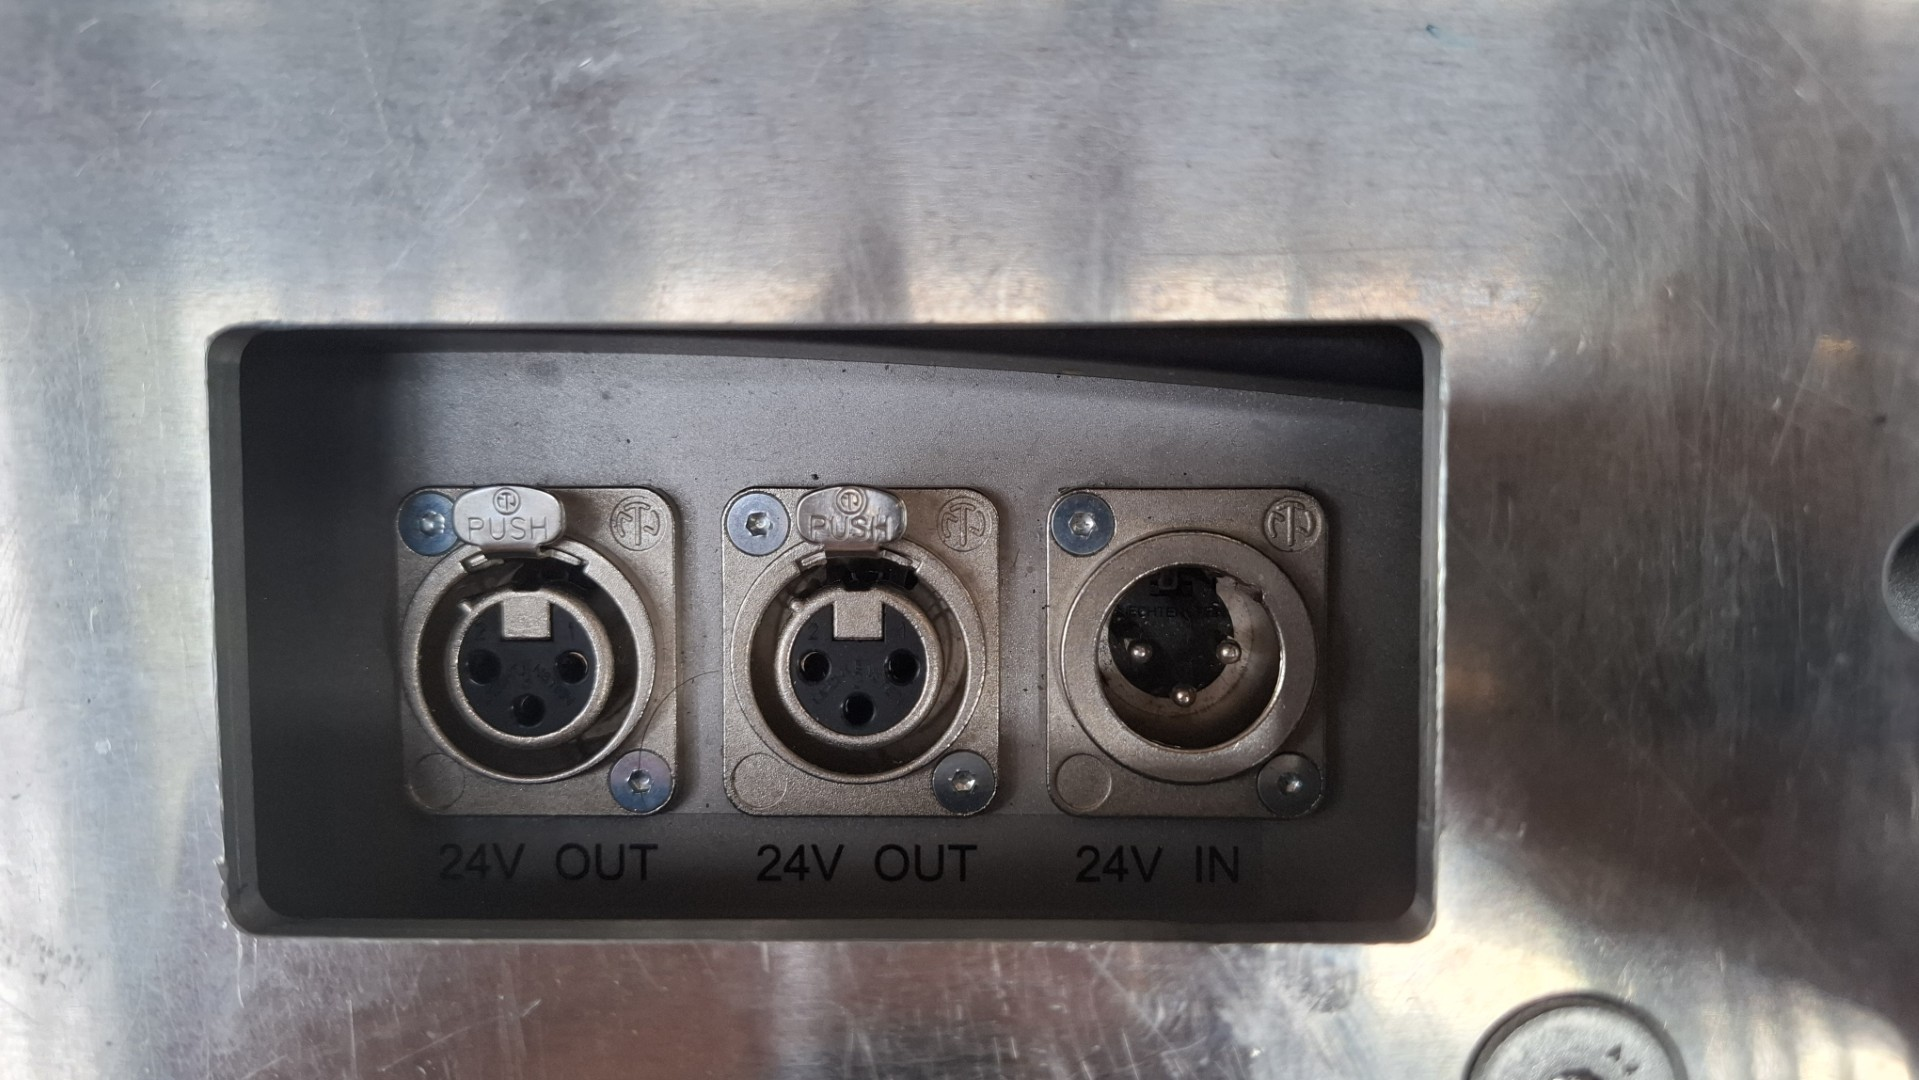
\includegraphics[width=\linewidth]{images/sec2/youbot_power.jpg}
            \caption{Image 1}
        \end{subfigure}
        \hfill
        \begin{subfigure}[t]{0.49\linewidth}
            \centering
            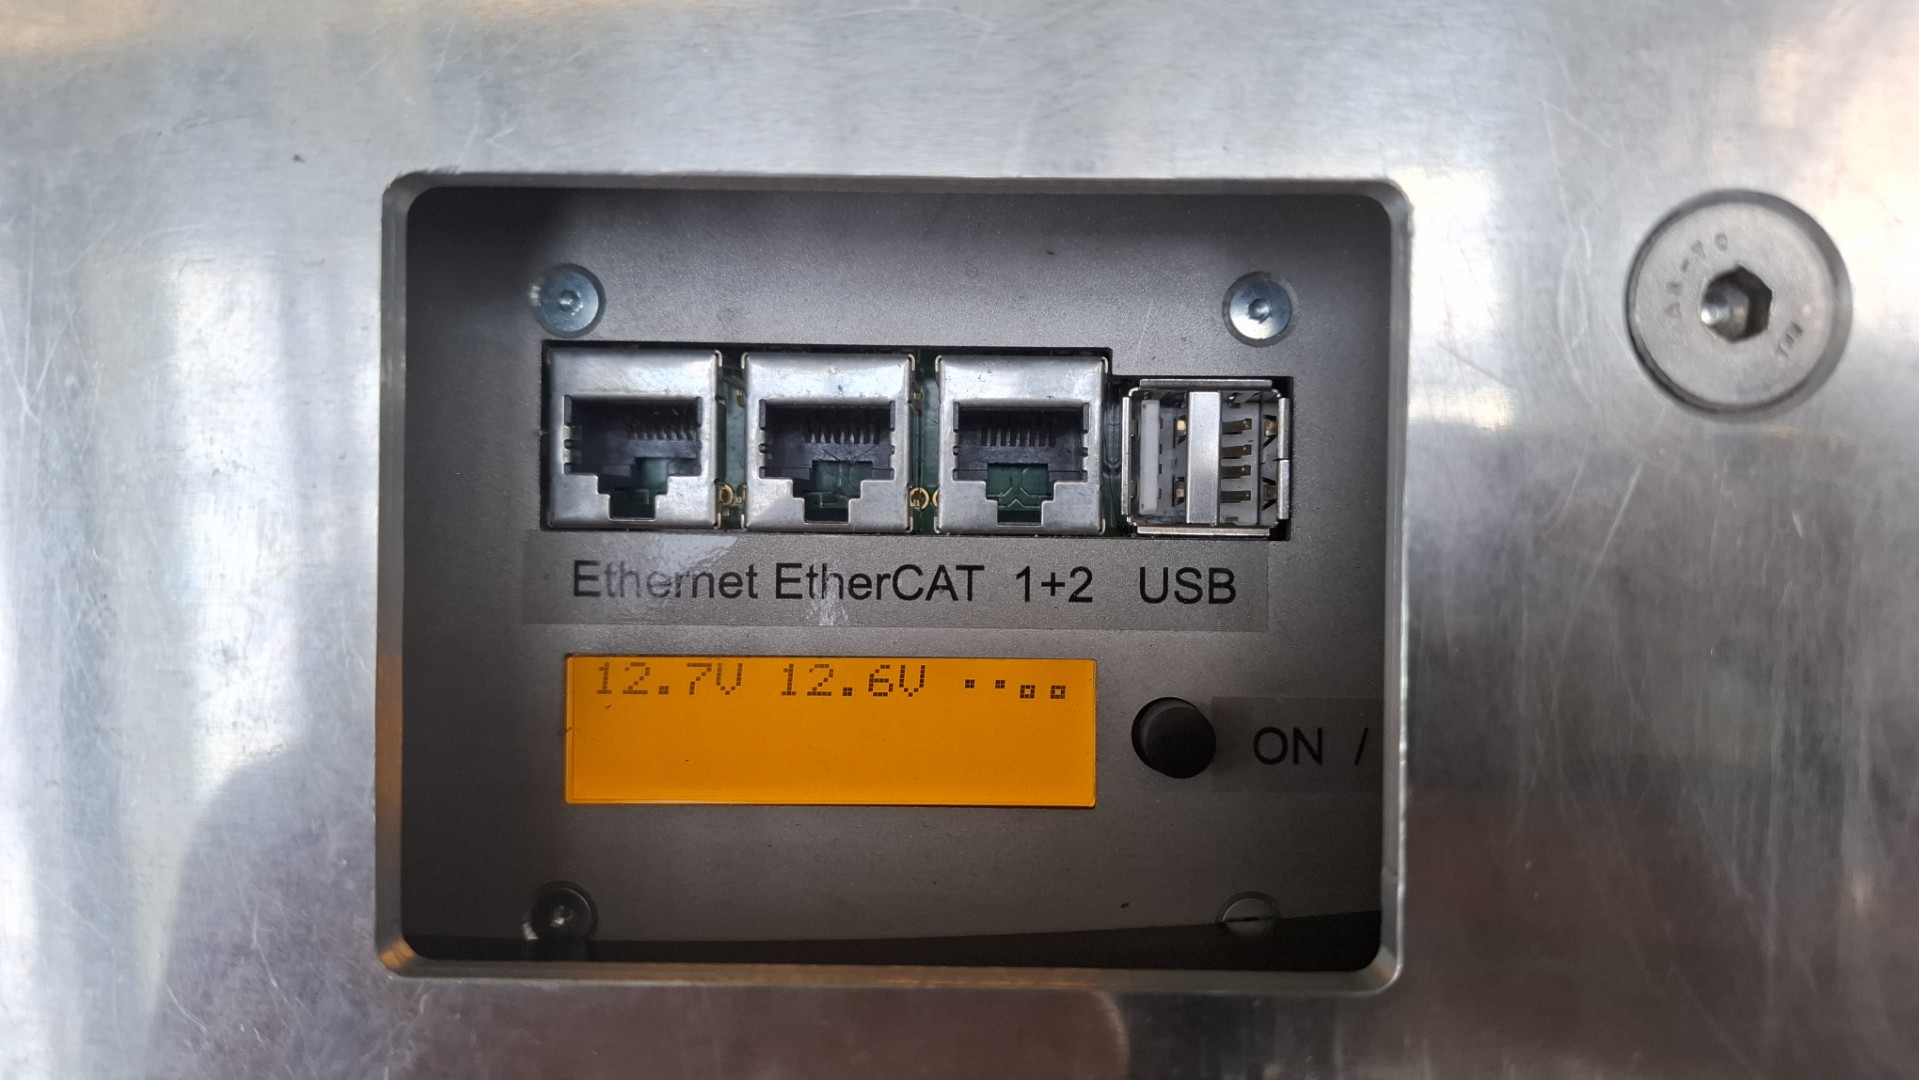
\includegraphics[width=\linewidth]{images/sec2/youbot_screen.jpg}
            \caption{Image 2}
        \end{subfigure}

        \vspace{0.5em}  % Space between rows

        % Row 2
        \begin{subfigure}[t]{0.49\linewidth}
            \centering
            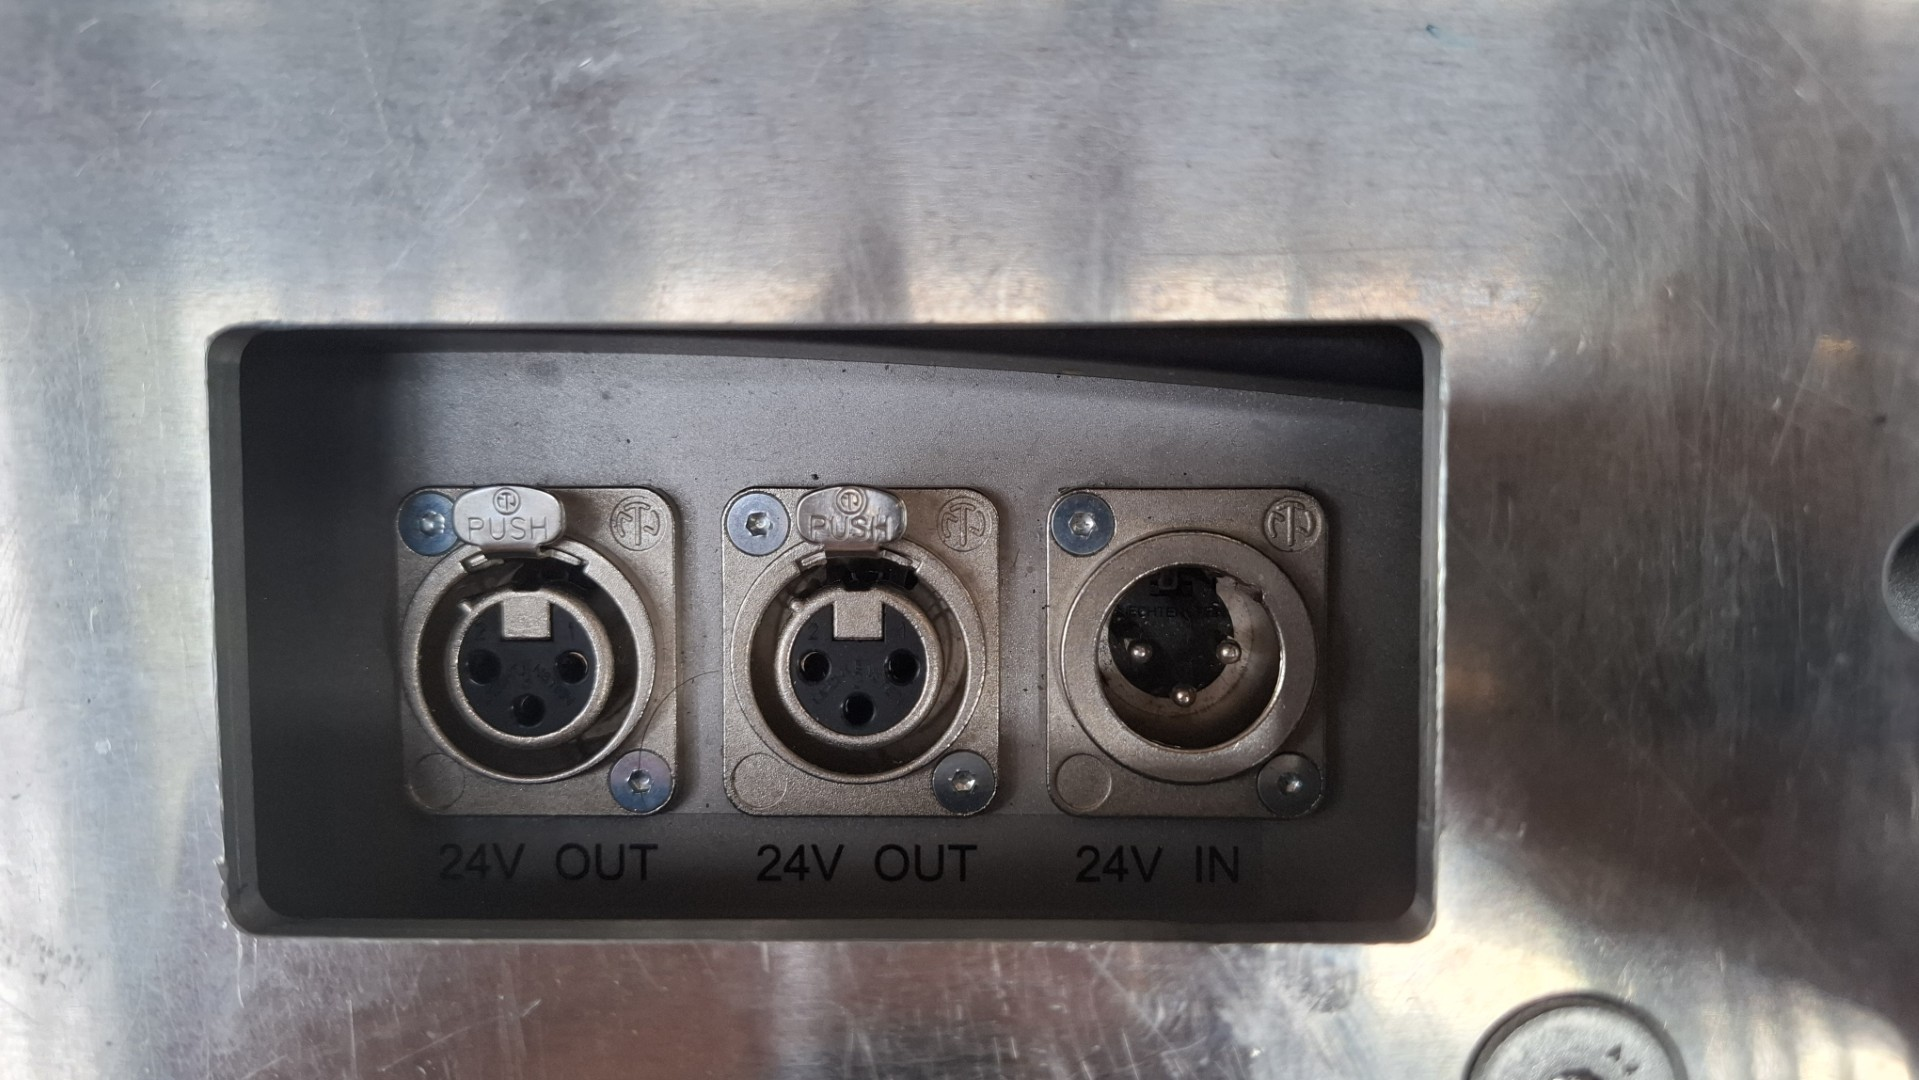
\includegraphics[width=\linewidth]{images/sec2/youbot_power.jpg}
            \caption{Image 3}
        \end{subfigure}
        \hfill
        \begin{subfigure}[t]{0.49\linewidth}
            \centering
            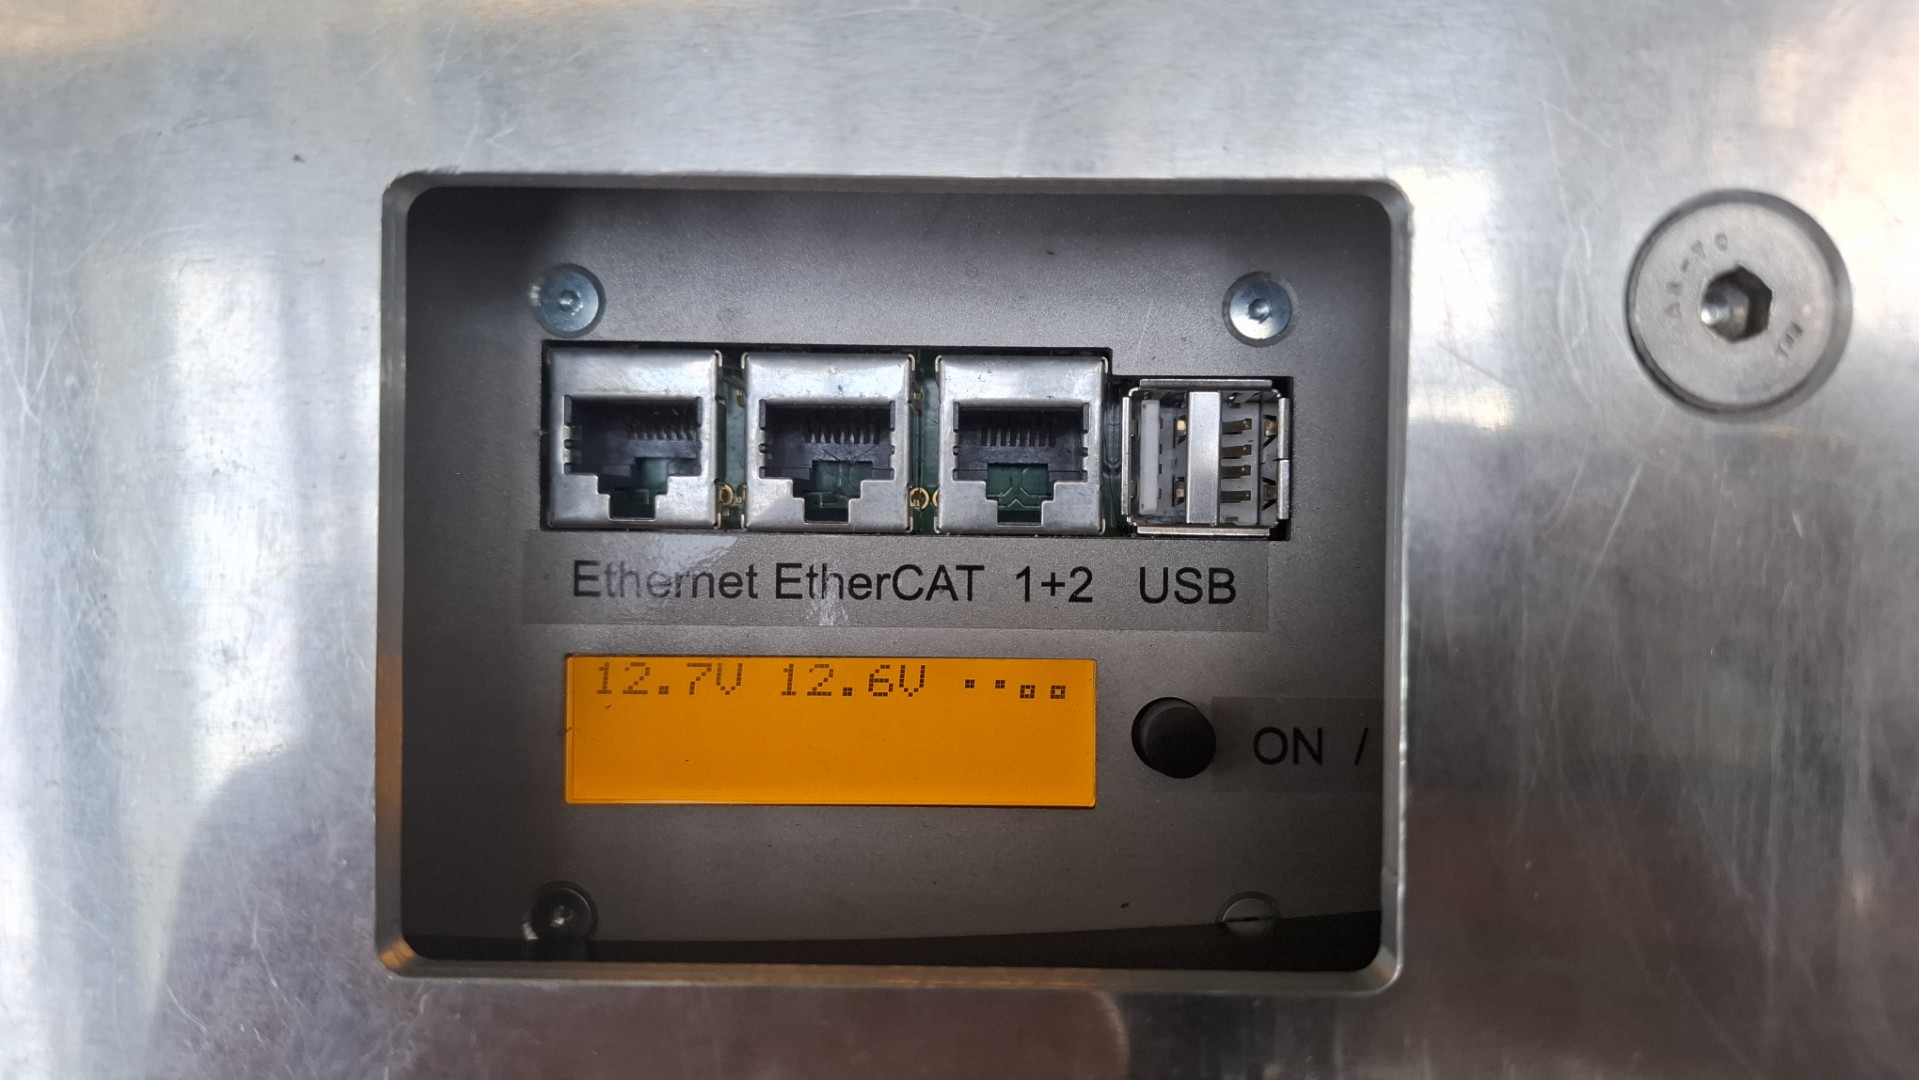
\includegraphics[width=\linewidth]{images/sec2/youbot_screen.jpg}
            \caption{Image 4}
        \end{subfigure}

        \caption{Four images tiled in a 2×2 layout}
        \label{fig:youbot-quad}
    \end{figure}

   

